% !TeX root = ../main.tex

\section{Introduzione}

\begin{frame}{Introduzione}
    \begin{columns}[onlytextwidth,t]
        \begin{column}{0.5\textwidth}
        
            \textbf{Necessità}:
            \begin{itemize}
                \item Innovazione
                \item Ottimizzazione
                \item Soddisfare i requisiti del cliente
                \item Tempi brevi di rilascio
                \item Accogliere le modifiche rapidamente
                \item Riuso del software
                \item Riduzione degli errori
                \item ...
            \end{itemize}
            
        \end{column}
        \begin{column}{0.5\textwidth}
        
            \textbf{Soluzione}:
            \begin{itemize}
                \item DevOps
                \item Applicazioni Multipiattaforma
            \end{itemize}
            
        \end{column}
    \end{columns}    
    
    \vspace{5mm}
    
    \textbf{Obiettivo}: Dimostrare l'efficacia della cultura DevOps e del paradigma multipiattaforma, adottati per lo sviluppo di applicazioni mobile
\end{frame}

\begin{frame}{DevOps}
    \begin{columns}[onlytextwidth]
        \begin{column}{0.45\textwidth}
        
            \textbf{Principi}:
            \begin{itemize}
                \item Comunicazione/Collaborazione
                \item Automazione
                \item Monitoraggio
            \end{itemize}
            
            \vspace{3mm}
            
            \textbf{Vantaggi}:
            \begin{itemize}
                \item Risparmio di tempo e risorse
                \item Tempi di consegna minori
                \item Maggiore qualità
            \end{itemize}
            
            \vspace{3mm}
            
            \textbf{Tecniche}:
            \begin{itemize}
                \item Continuous Integration
                \item Continuous Delivery
                \item Continuous Inspection
                \item ...
            \end{itemize}
            
        \end{column}
        \begin{column}{0.55\textwidth}
        
             \begin{figure}[H]
                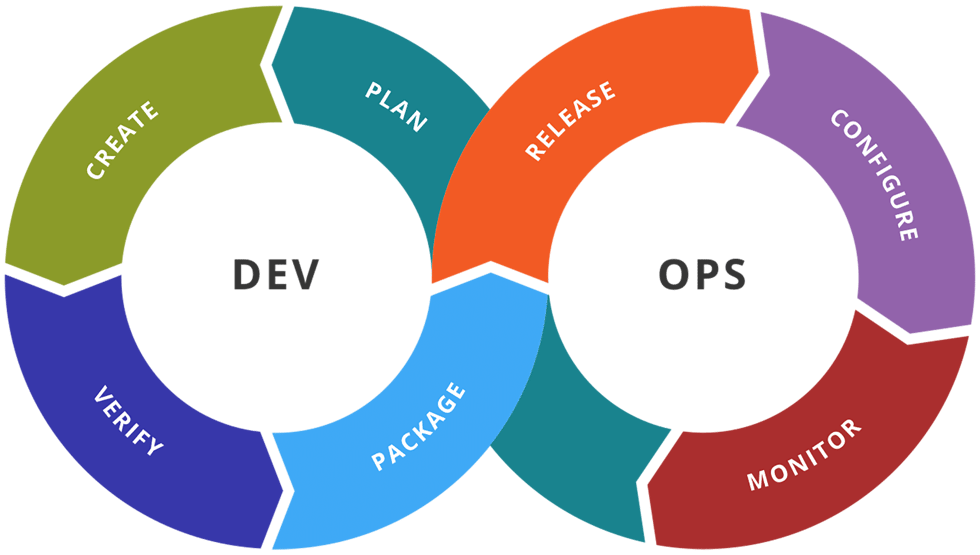
\includegraphics[width=1\textwidth]{img/Devops-toolchain.png}
            \end{figure}
            
        \end{column}
    \end{columns}
\end{frame}

\begin{frame}{Applicazioni Multipiattaforma}

    \textbf{Cross-piattaforma}:
    \begin{itemize}
        \item Condivisione/riuso totale del codice
        \item Performance limitate dovute alla presenza di uno strato software aggiuntivo di traduzione del codice
        \item Accesso limitato e con overhead alle funzionalità hardware del dispositivo dovuto alla presenza dello strato software aggiuntivo
        \item Frameworks: Ionic, Flutter, React Native, ...
    \end{itemize}
    
    \vspace{5mm}
    
    \textbf{Multi-piattaforma}:
    \begin{itemize}
        \item Condivisione/riuso della logica applicativa
        \item Performance elevate, equivalenti a quelle native
        \item Accesso completo e senza overhead alle funzionalità hardware del dispositivo
        \item Frameworks: \textbf{Kotlin Multiplatform Mobile}
    \end{itemize}
    
\end{frame}

\begin{frame}{Kotlin Multiplatform Mobile}
    \begin{columns}[onlytextwidth]
        \begin{column}{0.55\textwidth}
        
             \begin{figure}[H]
                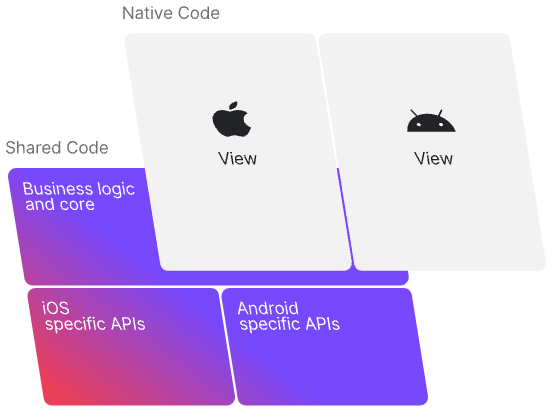
\includegraphics[width=1\textwidth]{img/kmm-stack-official.png}
            \end{figure}
            
        \end{column}
        \begin{column}{0.45\textwidth}
        
            \textbf{Caratteristiche}:
            \begin{itemize}
                \item Framework per lo sviluppo di applicazioni mobile multipiattaforma per Android e iOS
                \item Ancora non molto maturo (fase ``pre-stable'')
                \item Utilizzato in produzione da aziende come Netflix, Philips e VMware
                \item Il codice condiviso viene compilato in binari eseguibili direttamente dal dispositivo senza il bisogno di strati software aggiuntivi
            \end{itemize}
            
        \end{column}
    \end{columns}
\end{frame}